\documentclass[12pt]{article}

\usepackage{setspace}
\usepackage{minted}
\usepackage{fancyvrb}
\usepackage{listings}
\usepackage{graphicx}

\usepackage[margin=0.75in]{geometry}
\pagestyle{empty}

\def \name       {Enrique Gavidia}
\def \coursenum  {CSC 415.01}
\def \coursename {Operating Systems Principles}
\def \instructor {Prof. Murphy}
\def \semester   {Spring 2012}
\def \assignment {Homework \# 7}
\def \duedate    {May 9, 2012}

\newcommand {\mytilde} {$\sim$}
\newcommand {\comment}[1] {\textcolor{red}{#1}}
\newcommand {\filename}[1] {\flushleft \textbf{#1}}
\newcommand {\append}[2] {\section*{Appendix #1} \textsl{\large #2}}

\newcommand {\makecover} {
  \begin{titlepage}
    \begin{center}
      \LARGE{\coursenum, \semester \\ \coursename}\\
      \Large{\instructor}\\
      \vfill
      \textbf{\Huge \assignment}\\
      \vfill
      \Large{\name}\\
      \large{\duedate}
    \end{center}
  \end{titlepage}
}

\DefineVerbatimEnvironment {shelloutput} {Verbatim} {fontsize=\scriptsize, numbers=left, frame=lines, commandchars=\%\{\}}

\newcommand {\includesource}[2] {\inputminted[linenos, fontsize=\scriptsize, frame=lines]{#1}{#2}}
\newcommand {\includeoutput}[1] {\VerbatimInput[fontsize=\scriptsize, numbers=left, frame=lines, commandchars=\%\{\}]{#1}}

\begin{document}

\makecover

%---{ Main Content }--------------------------------------------------------------------
\section*{Assignment Description}
%For this assignment, we were to explore concurrency+parallelism using single and multiple core environments, through the monitoring 
%of performance when running concurrent programs. Our task was to implement a multi-threaded searching algorithm that partitions a
%large data set into a specified number of chunks, and searches them concurrently for a search key.  We then had to measure the performance
%of the algorithm in both Windows and Unix environments with Single and Multiple CPU cores.  The focus of the monitoring was to compare
%the advantages of running concurrent code in a parallel multi-core environment, as opposed to a single-core environment. To aid in this
%comparison, we graphed the performances of all the different systems as functions of the program's number of threads, versus the time
%they took to complete. The results supported the notion that multiple parallel processor systems are more efficient at executing concurrent 
%code than single core systems.

 
This code has been tested to work under \textsl{Windows}, \textsl{Gentoo Linux}, and \textsl{Mac OSX}.
The implementation for \textsl{Unix} is under \textbf{Appendix II}, and the \textsl{Windows} implementation is in \textbf{Appendix IV}. 
The \textsl{Pseudocode} outlining the design of both implementations is in \textbf{Appendix I}.
And the graphs for the outputs of the different systems are located under \textbf{Appendix VI}.


\section*{Design \& Implementation}
%The design of the program is fairly simple and straightforward; I wrote the implementations just as they ere outlined in the Pseudocode.
%The threads each search a separate partition of the data set, and store their results in another array, which is then searched for
%errors as it is being output to the user. In Unix there wasn't much trouble getting the algorithm to run and yield it's performance 
%results as expected, but for the Windows implementation however, there wasn't a straightforward way to truly accurately measure time in 
%microseconds with the Win32 API for the performance measurement portion of the assignment. Instead, the API provides access to the CPU's 
%internal clock counter, which is what I used to then extrapolate a simple approximation of the algorithm's elapsed time in microseconds.  
%Another obstacle with the Windows implementation was the limited range of the platform's \texttt{rand()} function, which is prone to causing 
%many 'error' results with duplicate keys at the array sizes we were dealing with. The array's size of $2^{18}$ was roughly an order of magnitude 
%larger than the largest value produced by the \texttt{rand()} function, so in order to minimize the possibility of errors while still maintaining 
%a reasonable chance for the array to contain the search key, I multiplied the results of two calls to \texttt{rand()} together, and restricted 
%their domain to twice the size of the array; i.e. 2($2^{18}$).


\section*{Results}
As for the results of the performance tests, the single-core systems performed as expected, handling the algorithm with 1 thread better than with multiple threads, but the Windows single-core machine seemed to have experienced a noticeably higher spike when attempting to run 4 or more threads. Both of the multi-core tests were performed on Dual-core systems, and both performed about the same in handling multiple threads better than the single-core system.


\section*{Improvements}
Like for the last assignment, I would switch to using a linked-list instead of the array for the generated values to improve memory usage. Additionally, instead of storing and keeping
track of the entire sorted array at the end, I could switch to using a 2-item array for storing the \textsl{current} and \textsl{previous} values returned from the \texttt{get_next} function,
which is all that should be needed to determine whether any of the values are not in sorted order; implementing this should cut down on memory usage a great deal.


%---{ Appendices }-----------------------------------------------------------------------
%\newpage

%----{ Unix }--------------------------------------------------------------------------

\append{I} {Pseudocode}
\begin{scriptsize}
\begin{verbatim}
int threads[];
int array[];
int array_size;
int sorted_array[];

semaphore sem;

sort_partition() {
    // sort array
    P(sem);
}

main() {

    // initialize random array...

    initialize_semaphore(s);

    for (thread in threads) {
        start_thread(thread, sort_partition)
    }

    for (thread in threads) {
        V(sem);
        end_thread(thread);
    }

    // check to make sure everything has been sorted right
    for (i = 0; i < array_size; i++) {
        sorted_array[i] = get_next();

        assert(sorted_array[i] >= sorted_array[i-1], "ERROR: Array is not sorted right");
    }
}
\end{verbatim}
\end{scriptsize}


\append{II} {Unix Source Code}
\includesource{c}{unix_sort.c}

\append{III} {Unix Output}
\filename{Single-core}
\includeoutput{output/unix_sort_singlecore.txt}

\filename{Multi-core}
\includeoutput{output/unix_sort_multicore.txt}

%----{ Windows }--------------------------------------------------------------------------
\append{IV} {Windows Source Code}
\includesource{c}{win_sort.c}

\append{V} {Windows Output}
\filename{Single-core}
\includeoutput{output/win_sort_singlecore.txt}

\filename{Multi-core}
\includeoutput{output/win_sort_multicore.txt}

\append{VI} {Graphs}
% Time (Y) vs # of Threads (x)


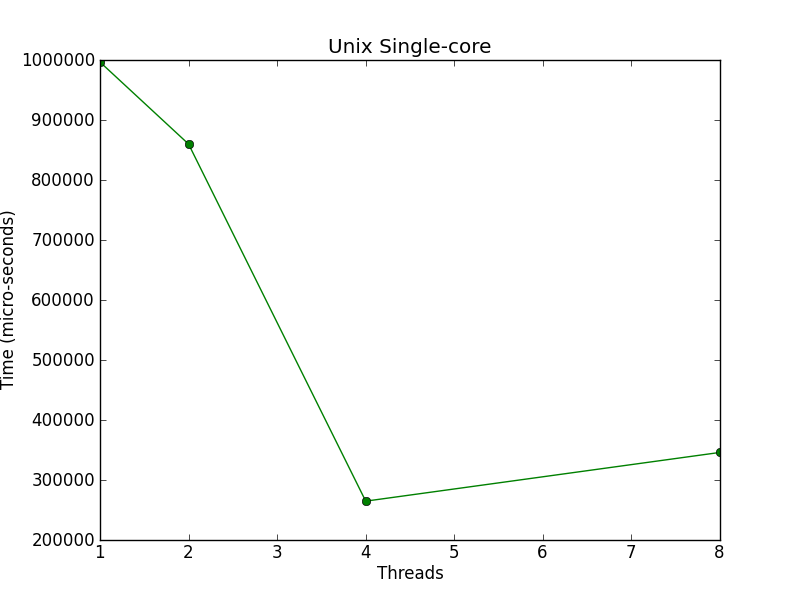
\includegraphics[scale=0.4]{output/graphs/unix_singlecore.png} 
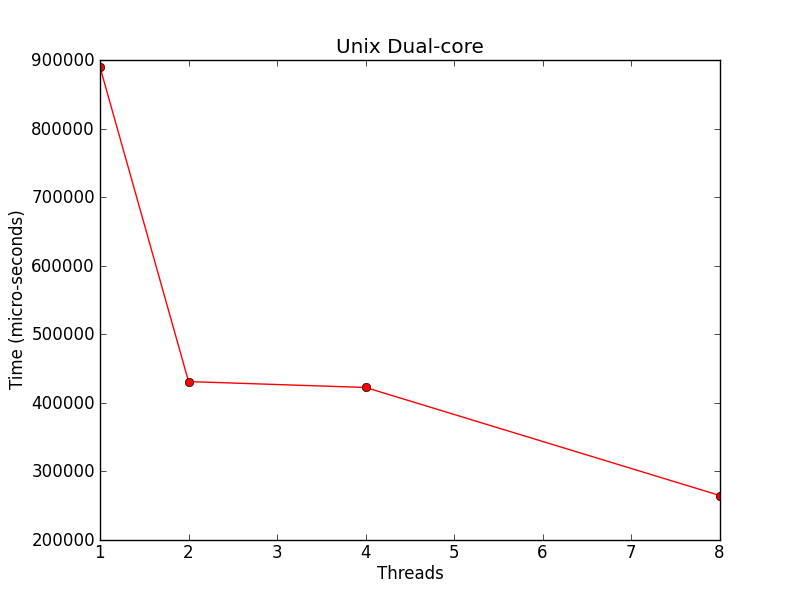
\includegraphics[scale=0.4]{output/graphs/unix_multicore.png}
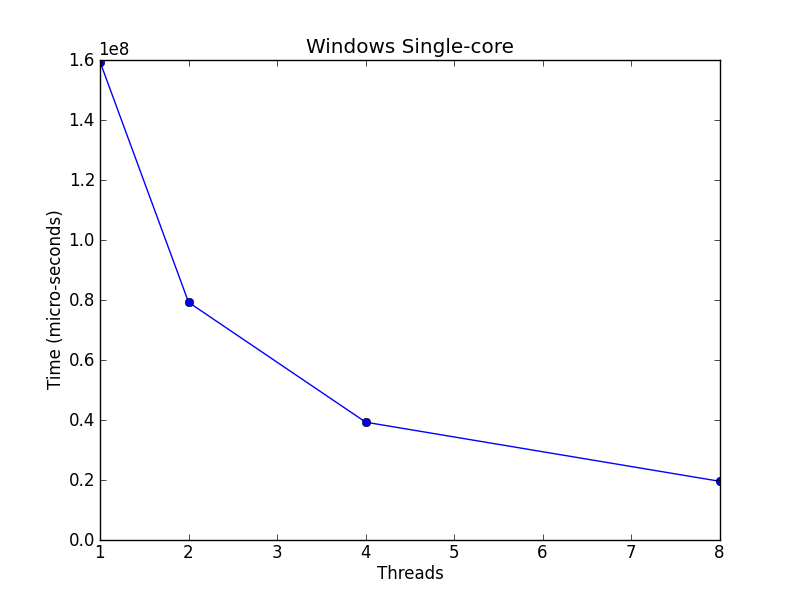
\includegraphics[scale=0.4]{output/graphs/win_singlecore.png} 
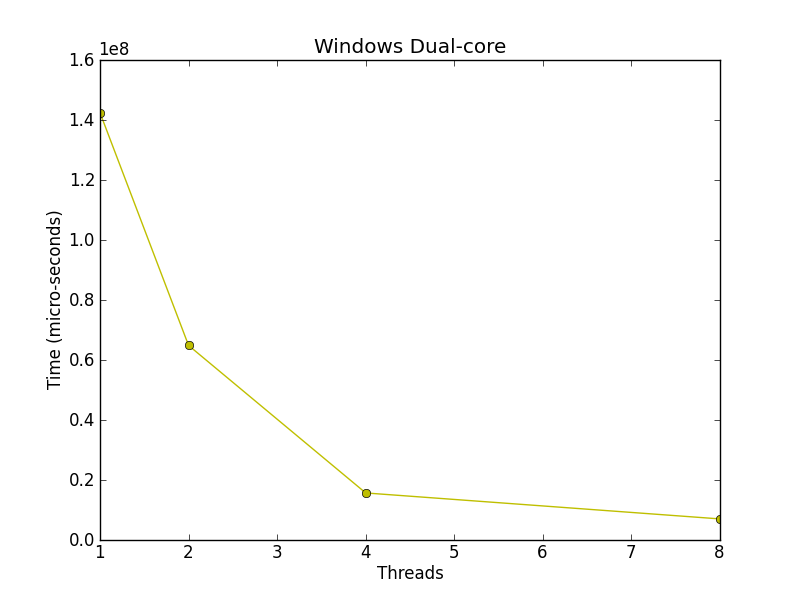
\includegraphics[scale=0.4]{output/graphs/win_multicore.png}


\end{document}
